\chapter{Technische Realisation}

\section{Aufgabenbereiche}

    % Welche Komponenten müssen technisch realisiert werden? 


    % Siehe Technische Daten

    % Beschreibung der prototypischen Realisierung, Vorgehensweise und
    % Beschreibung einzelner Schritte


    % Beschreibung der prototypischen Realisierung, Vorgehensweise und  Beschreibung einzelner Schritte
    % Verweise auf das Projekt-Repository in dem weitere Projekt-Artefakte zu finden sind (s.u.).






    Die technischen Aspekte des Gerippten lassen sich grob in folgende Teilbereiche aufgliedern:

    \begin{itemize}
        \item Beleuchtung der Tonnenaußenwand inklusive Animation der Lichteffekte sowie Beleuchtung des Flaschenrings
        \item Sensorik zur Detektion von Flaschen im Flaschenring
        \item Detektion von Gegenständen die in den Behälter geworfen werden
        \item Messung des Füllstandes
        \item Verkablung der Sensorik und der LEDs.
        \item Austausch von Informationen zwischen mehreren Endgeräten
        \item Verarbeitung der Sensordaten und Ansteuerung der Beleuchtung
    \end{itemize}

    In den nachfolgenden Kapiteln werden die zur Realisierung der verschiedenen Teilaspekte genutzten Komponenten beschrieben und diskutiert.


    \begin{figure}[h]
        \begin{center}
            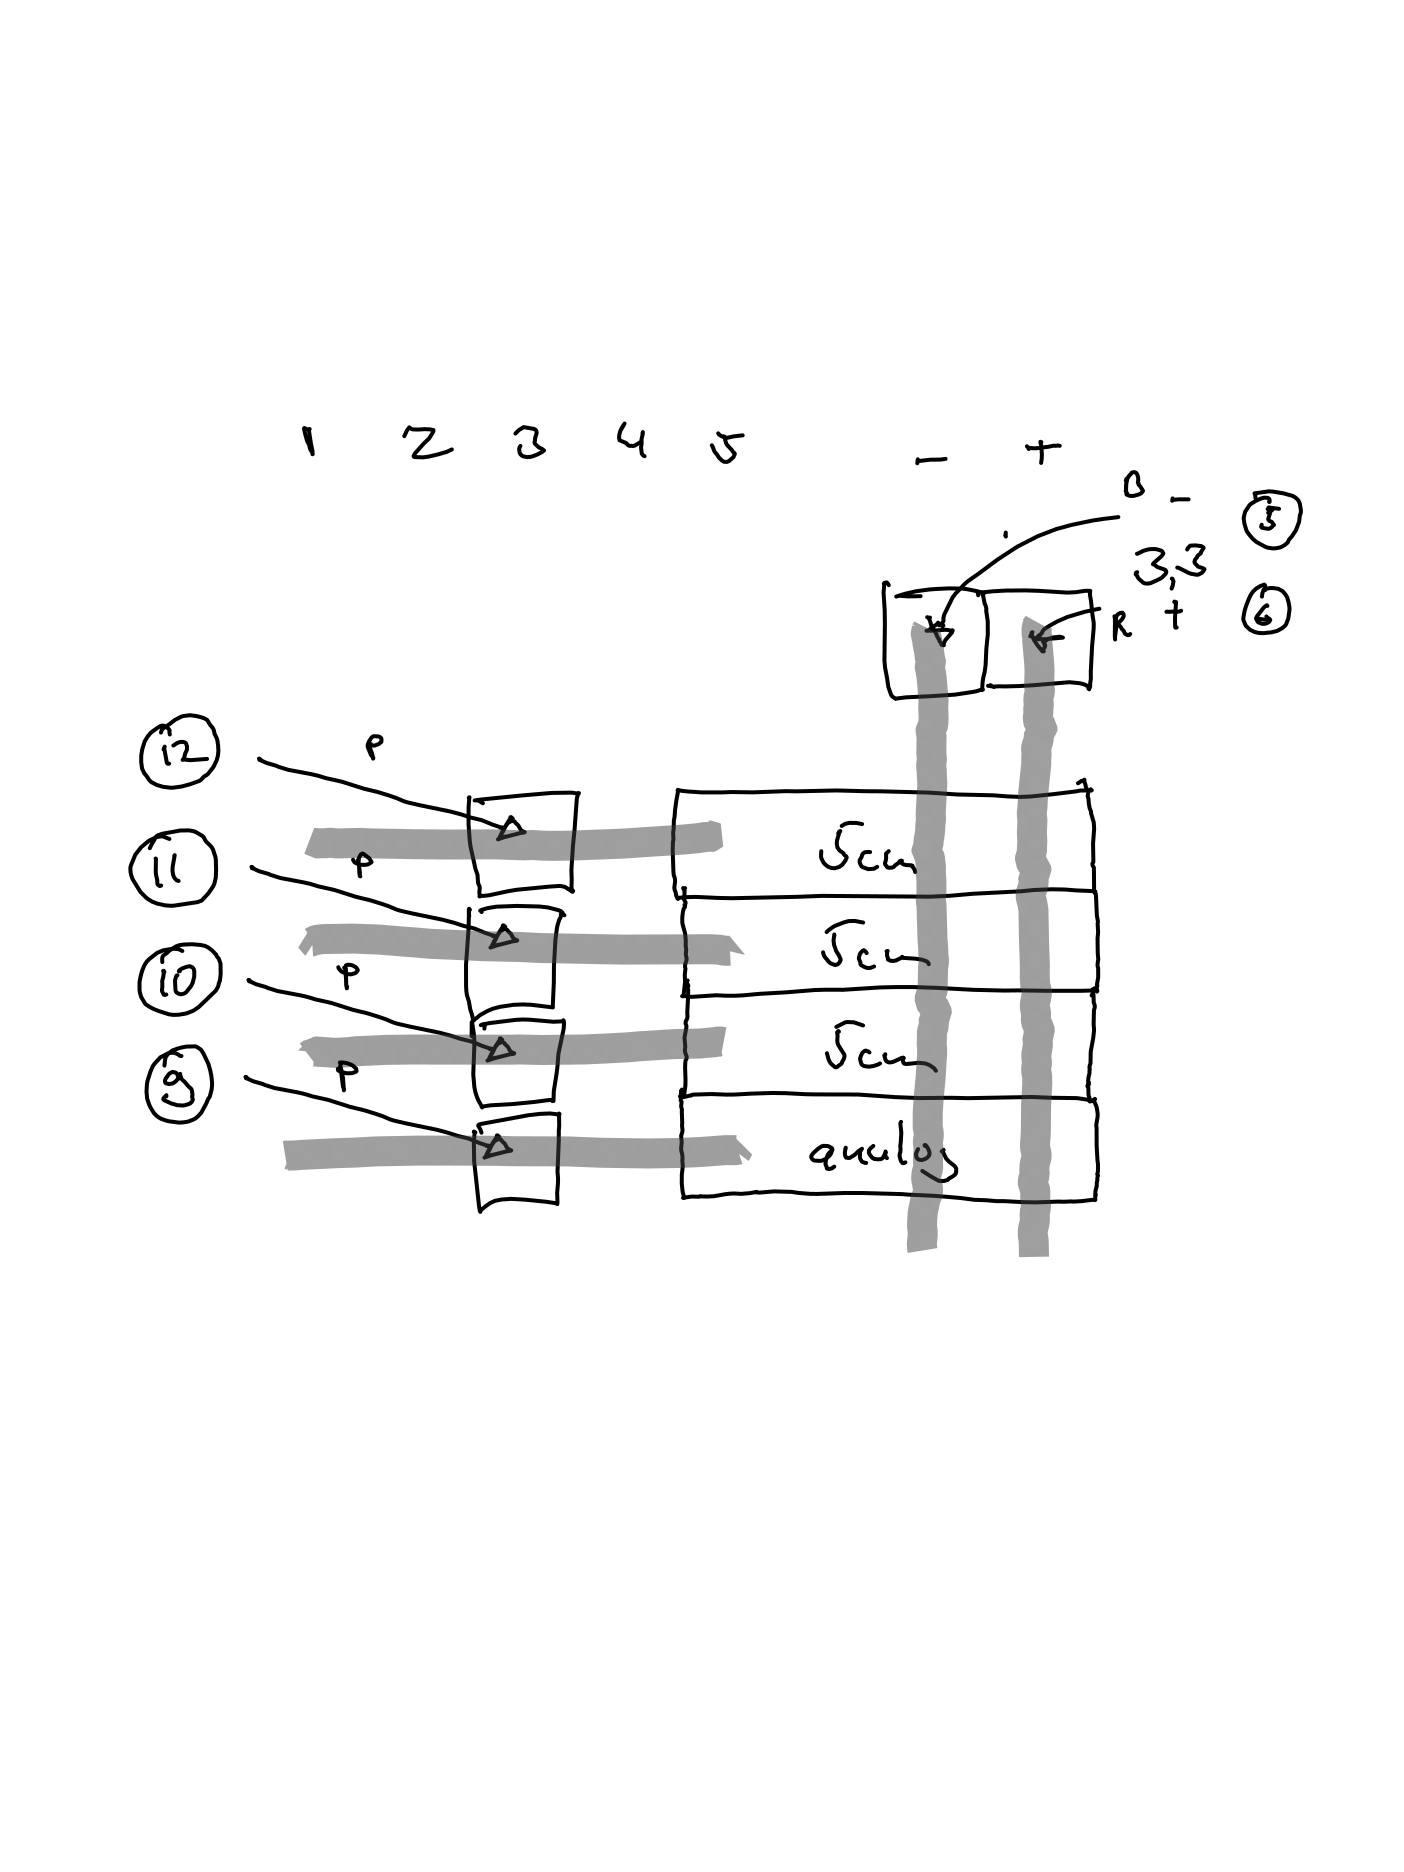
\includegraphics[width=9cm]{media/03_technical_implementation/header_1.png}
        \end{center}
        \caption{Caption}
        \label{fig:header_1}
    \end{figure}

    \begin{figure}[h]
        \begin{center}
            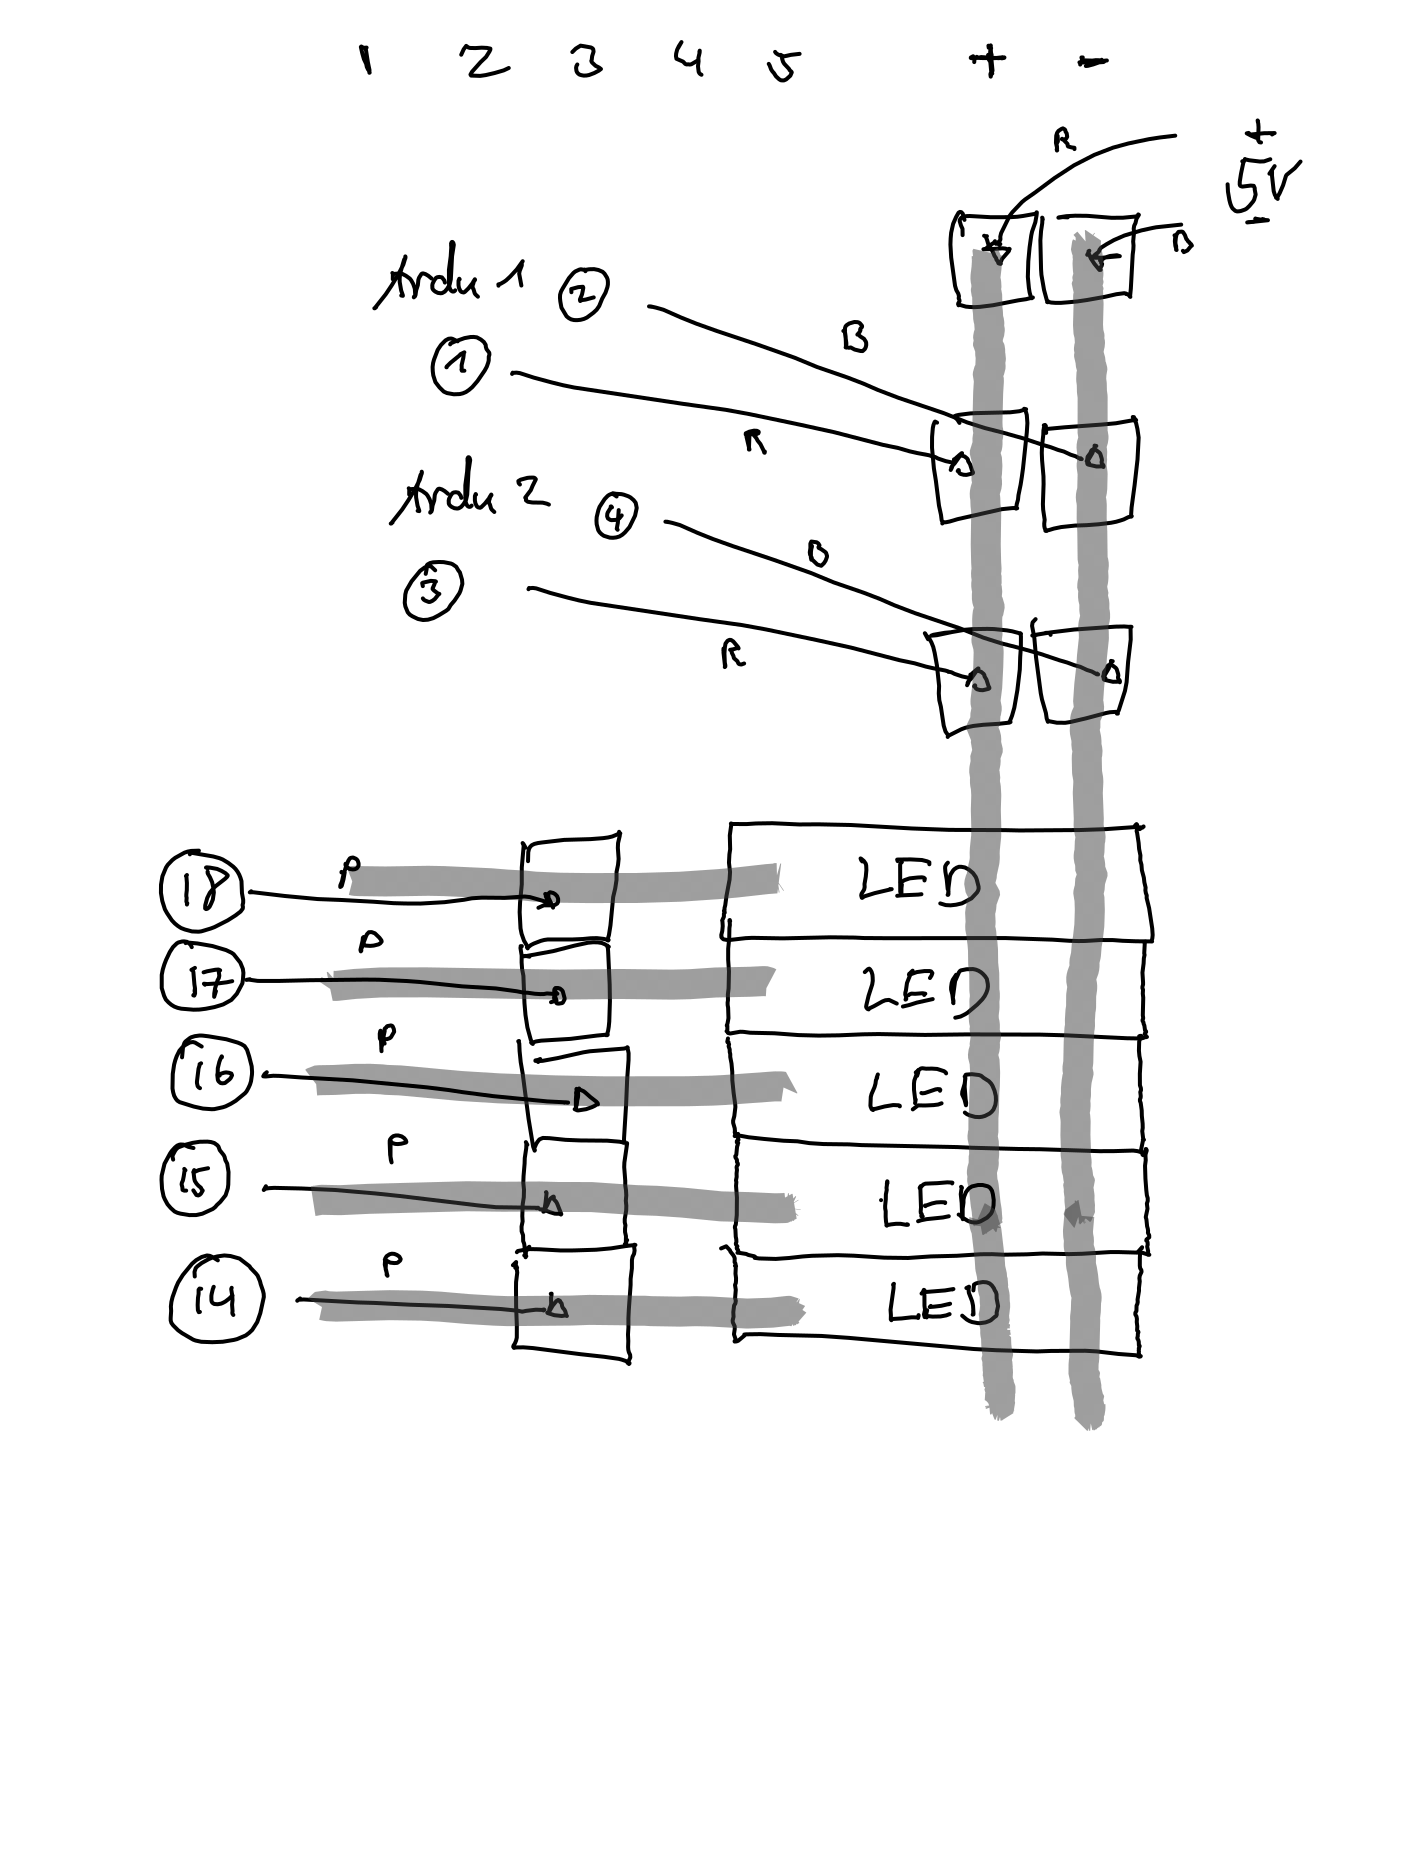
\includegraphics[width=9cm]{media/03_technical_implementation/header_2.png}
        \end{center}
        \caption{Caption}
        \label{fig:header_2}
    \end{figure}



\addtocontents{toc}{\protect\setcounter{tocdepth}{1}}

\section{Mikrocontroller}
    \subsection{Diskussion}
        Warum Arduino

    \subsection{}
        C++ \& PlatformIO

\section{Beleuchtung}
    \subsection{Diskussion}

    \subsection{Implementation}

        \begin{figure}[H]
            \begin{center}
                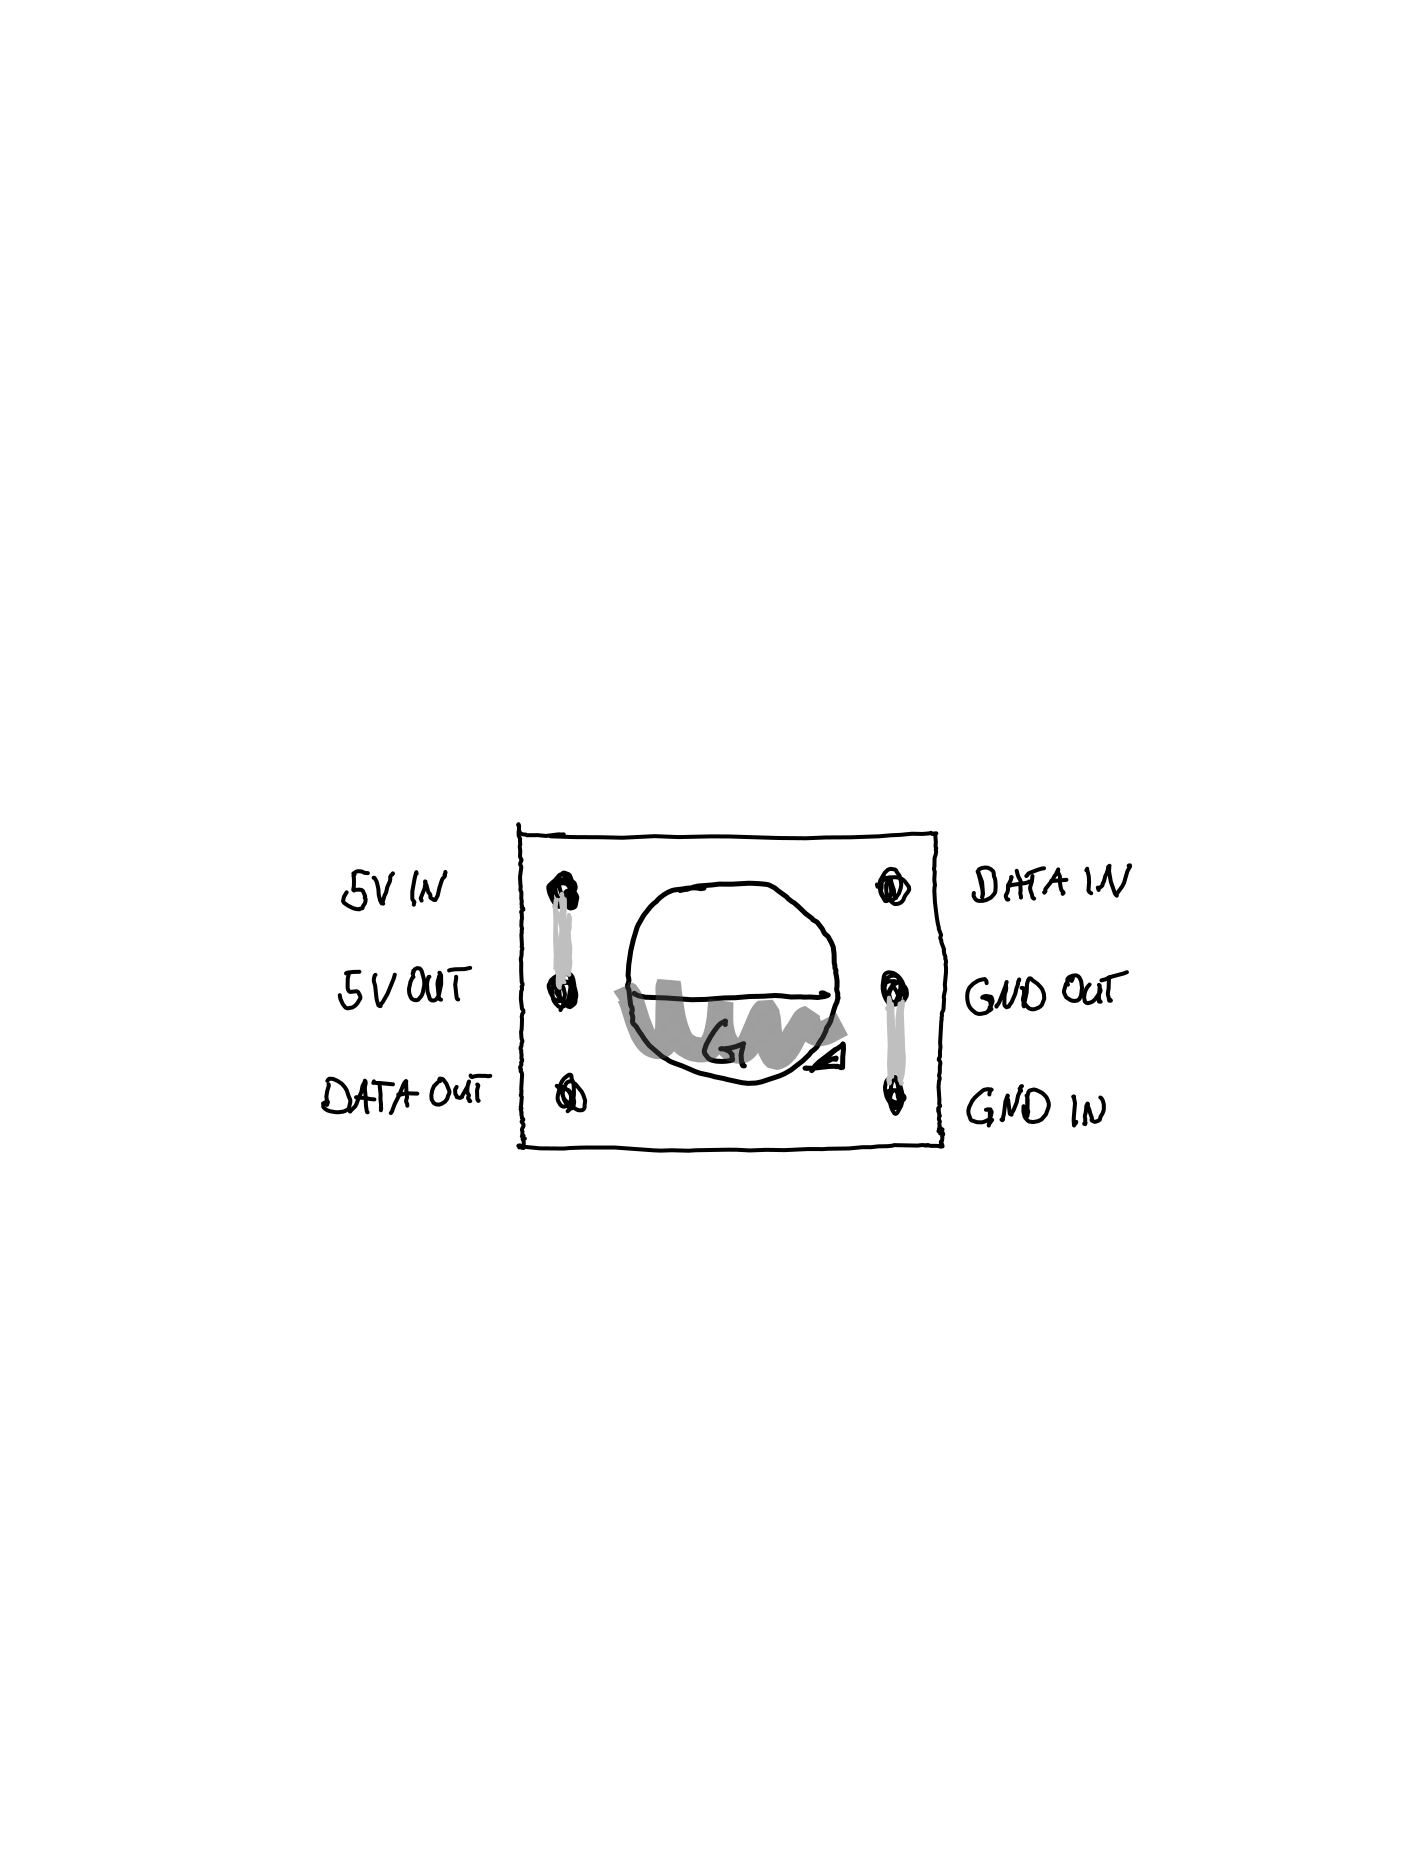
\includegraphics[width=7cm]{media/03_technical_implementation/leds_2.png}
            \end{center}
            \caption{Zeichnung Pin Belegung der NeoPixel SK6812RGBW}
            \label{fig:leds_2}
        \end{figure}
    
        \begin{figure}[H]
            \begin{center}
                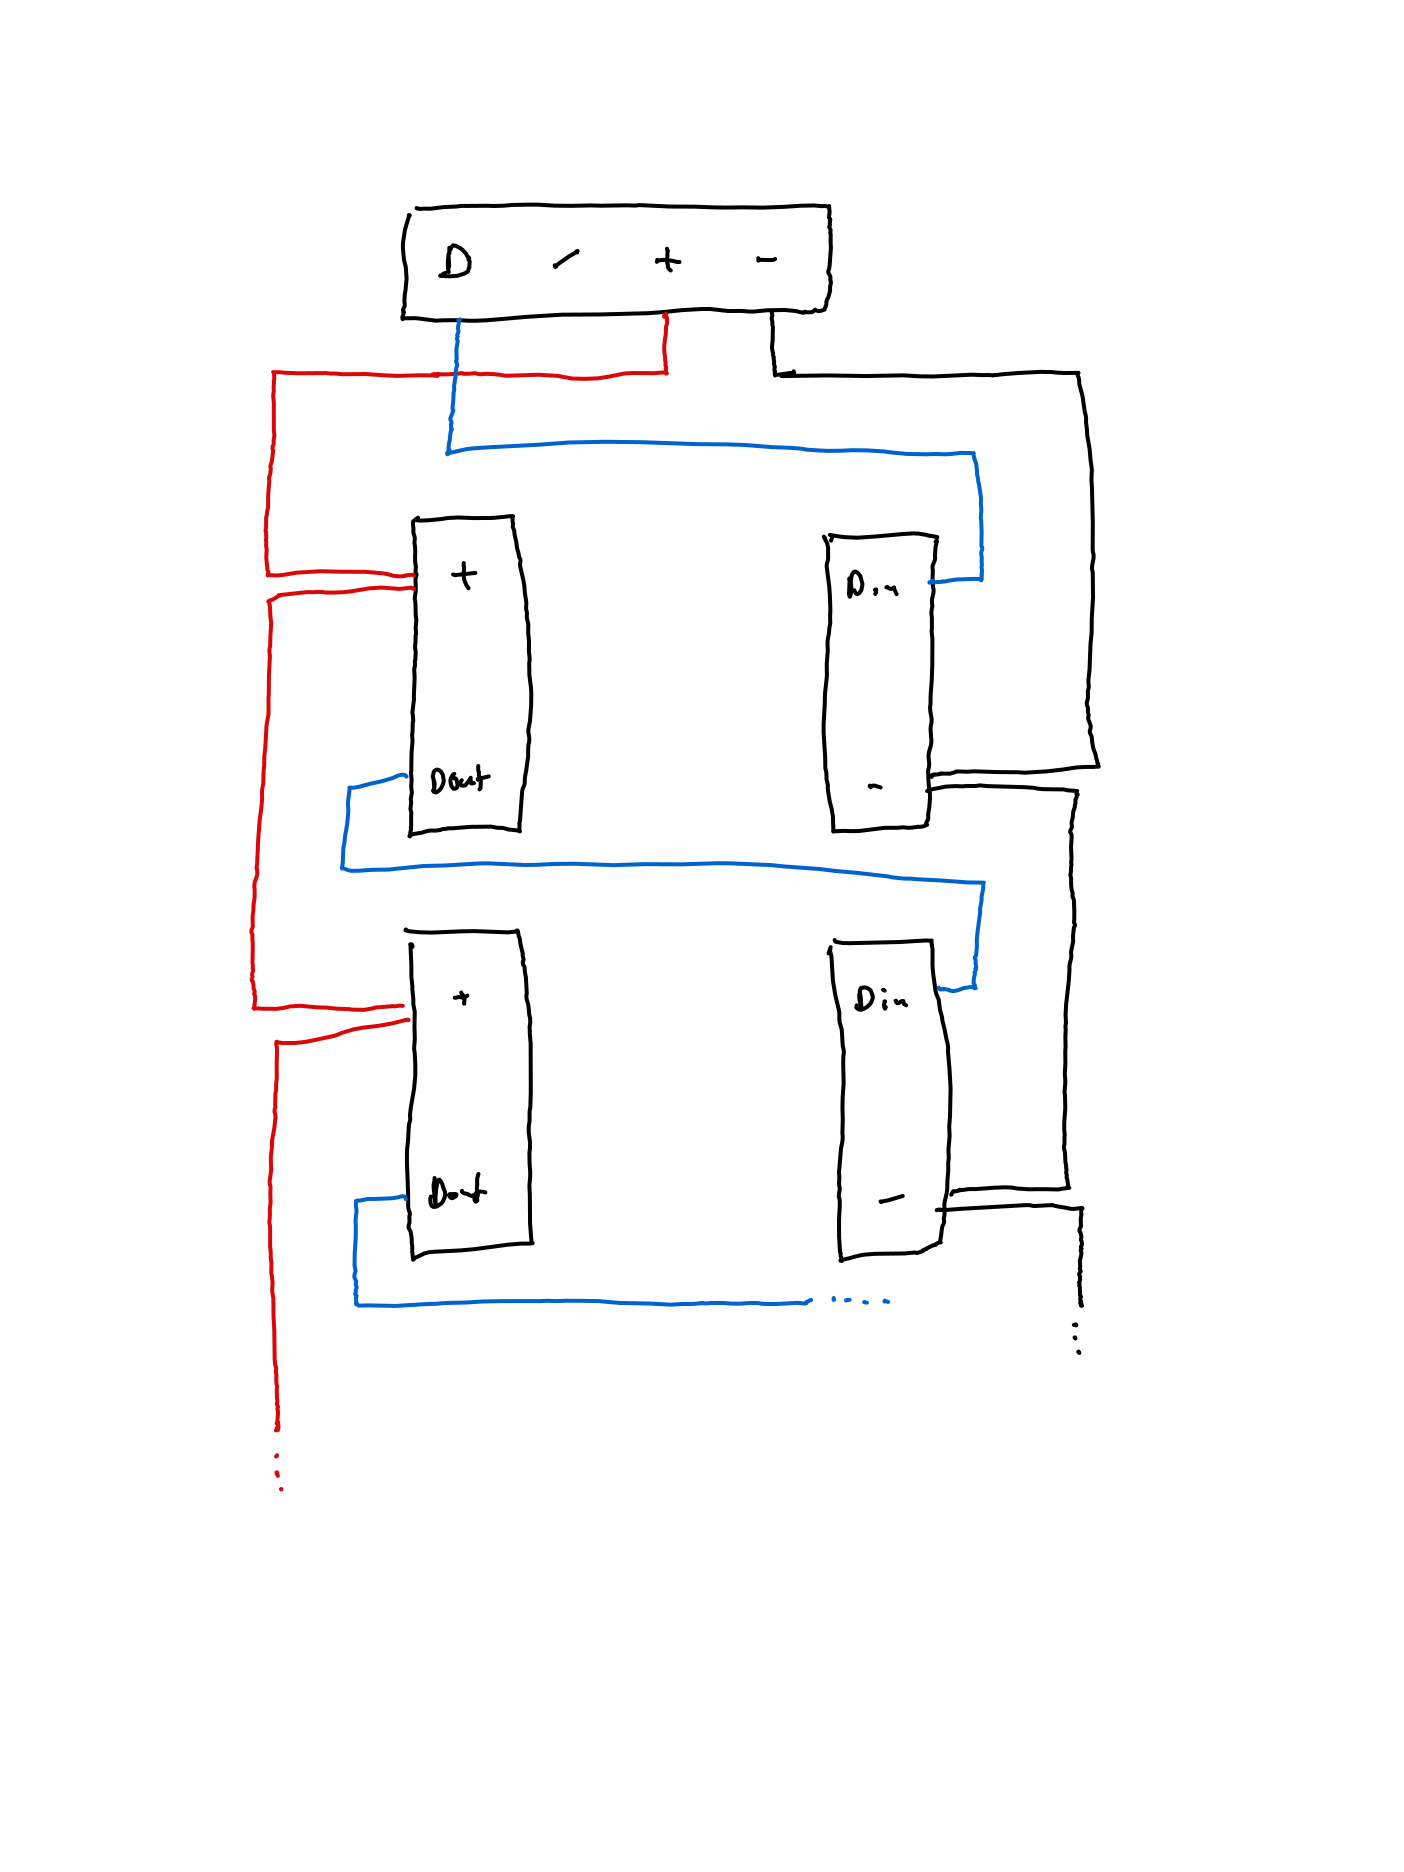
\includegraphics[width=7cm]{media/03_technical_implementation/leds_1.png}
            \end{center}
            \caption{Caption}
            \label{fig:leds_1}
        \end{figure}

        \begin{figure}[H]
            \begin{center}
                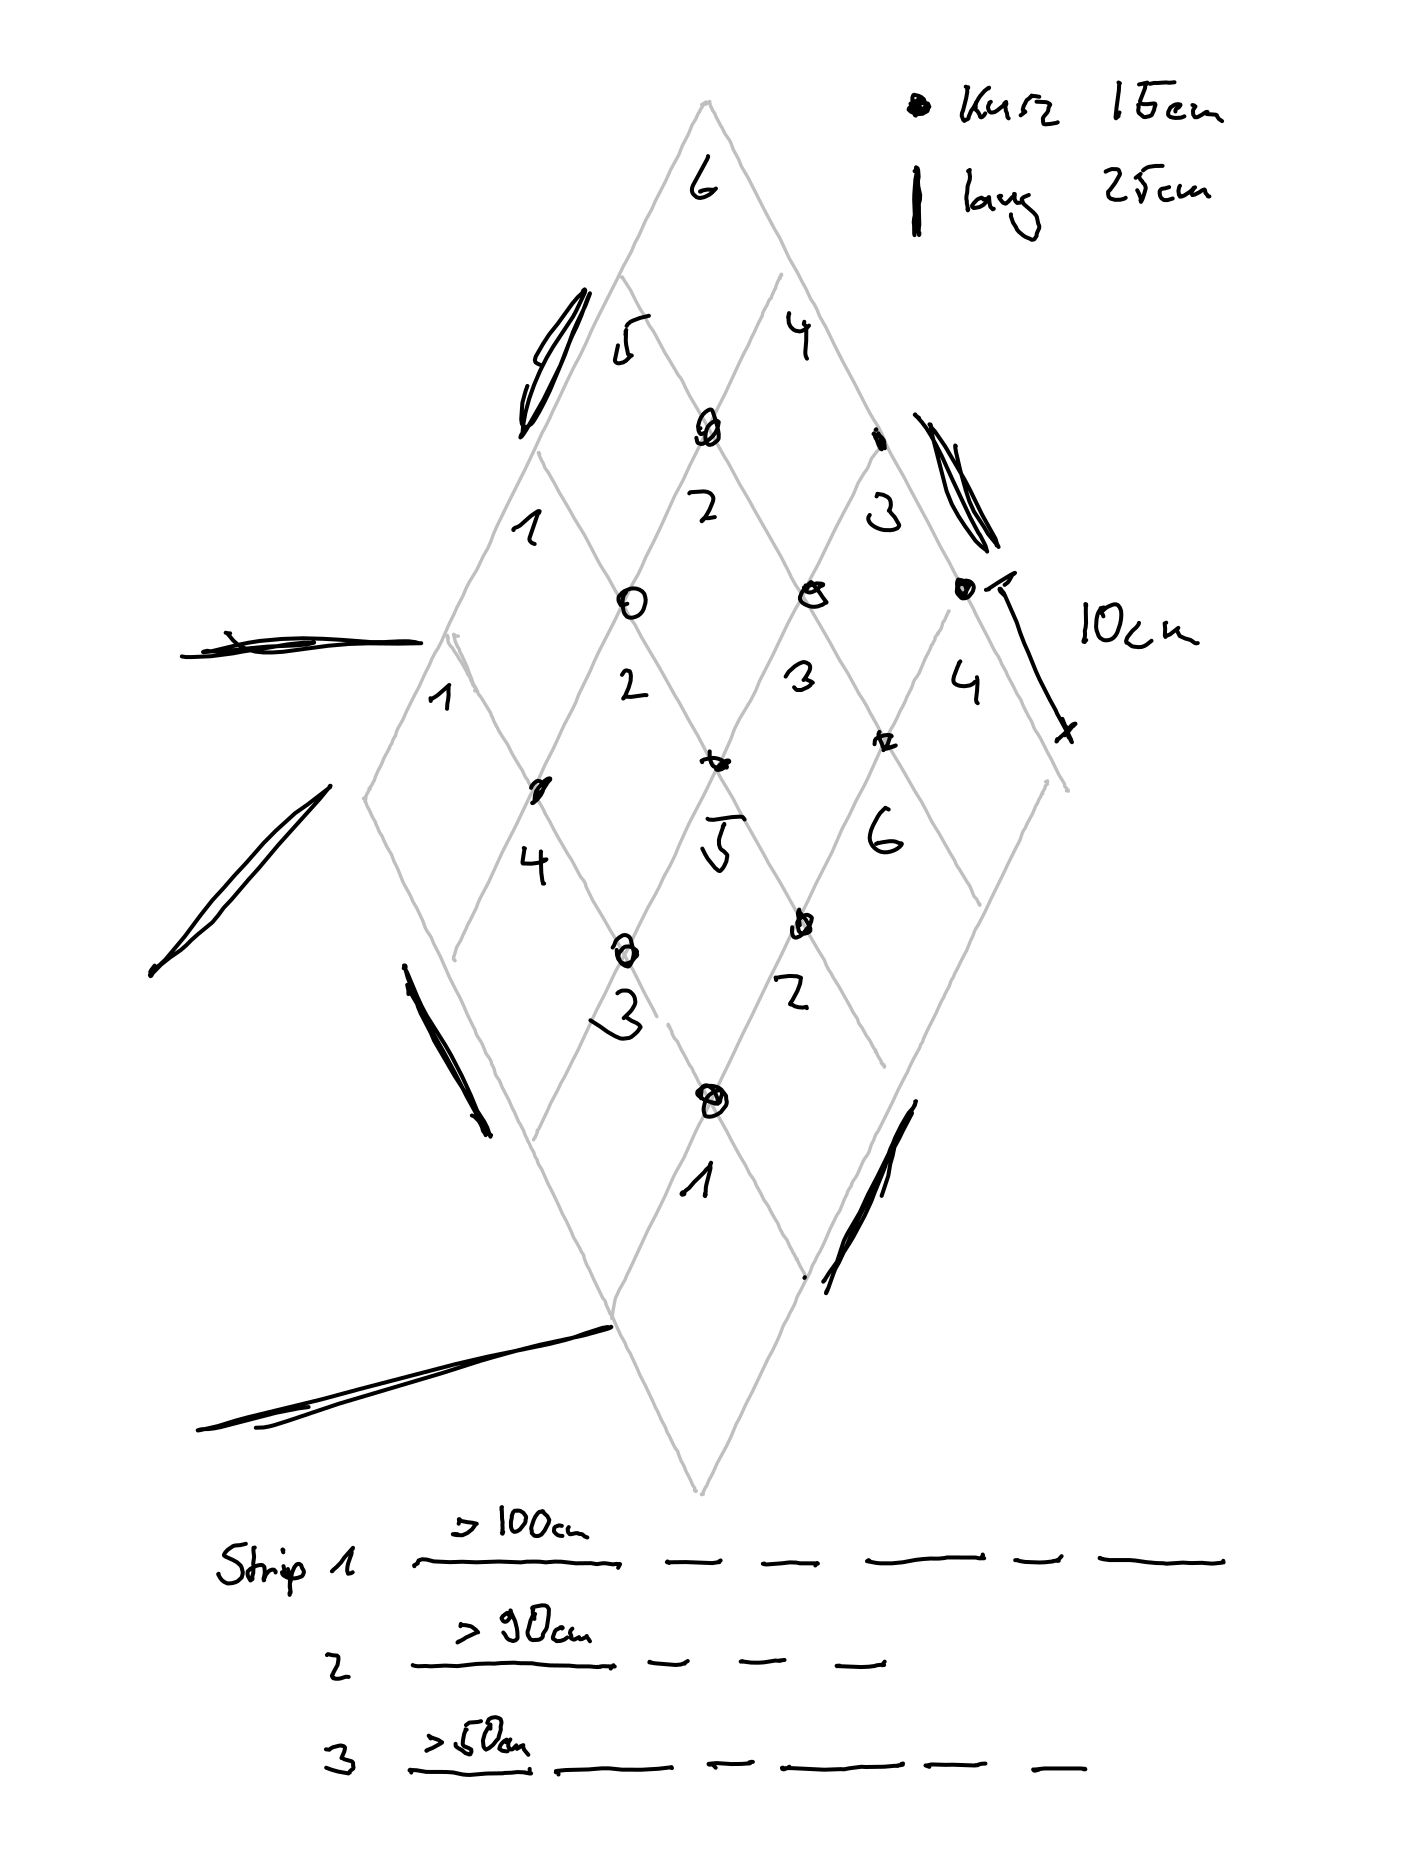
\includegraphics[width=12cm]{media/03_technical_implementation/leds_3.png}
            \end{center}
            \caption{Caption}
            \label{fig:leds_3}
        \end{figure}




\section{Animation}
    \subsection{Diskussion}

    \subsection{Implementation}

\section{Einwurferkennung}
    \subsection{Diskussion}
        Ein wichtiger Punkt bei der Realisierung der Einwurfserkennung ist, dass nur Gegenstände erkannt werden sollen, die gänzlich in den Behälter geworfen wurden und nicht wieder herausgezogen werden, wie es beispielsweise beim Hereinhalten einer Hand in den Behälter der Fall ist. Um dies zu implementieren muss der Gegenstand auf mindestens zwei übereinanderliegenden Ebenen detektiert werden. Wird auf der oberen Ebene der Gegenstand erkannt, wird ein möglicher Einwurf detektiert. Jedoch erst wenn die obere ebene keinen Gegenstand mehr detektiert, während die untere Ebene diesen weiterhin detektiert ist der Einwurf des Gegenstandes abgeschlossen. Sollte der Gegenstand hingegen zuletzt lediglich auf der oberen Ebene detektiert werden, so wurde er wieder aus dem Behälter herausgezogen und somit wird dies nicht als Einwurf gewertet.\\

        Die Realisierung der zwei Detektionsebenen durch zwei einzelne Sensoren oder Lichtschranken hat jedoch das Problem zur Folge, dass die beiden Sensoren miteinander interferieren, wenn sie die gleiche Lichtwellenfrequenz nutzen, was zur Folge hat, dass eine genaue Abgrenzung zwischen den Ebenen nicht möglich ist. Zur Realisierung dieser Funktion ist es deshalb notwendig Sensoren zu verwenden, die unterschiedliche Lichtwellenfrequenzen verwenden, oder es muss ein Sensor verwendet werden, der die Möglichkeit bietet Objekte in einem dreidimensionalen Bereich zu detektieren, statt nur auf einer bestimmten Ebene zu messen.\\

        Bei der Recherche nach zur Verfügung stehenden Komponenten fiel die Wahl letztlich auf den Mini dToF Imager TMF8821 von SparkFun. Dabei handelt es sich um einen so genannten direct Time of Flight Sensor. Damit ist ein Sensor gemeint, welcher viele kurze Lichtimpulse aussendet und die reflektierten Lichtimpulse wieder detektiert. Um die Entfernung zum Objekt zu bestimmen, welches den Lichtimpuls reflektiert hat, wird die Zeit gemessen, die zwischen der Aussendung des Lichtimpulses und der Detektion des reflektierten Lichtimpulses verstreicht. Eine Besonderheit des TMF8821 ist, dass dieser einen in mehrere Felder aufgeteilten Messbereich besitzt. So kann die Entfernung zu einem Gegenstand beispielsweise in 9 verschiedenen Messbereichen, aufgeteilt auf ein 3x3 Quadrat, gemessen werden. Der Messbereich kann Softwareseitig angepasst werden und somit sind verschiedene Messwinkel und Submessbereiche in den Ausprägungen 3x3, 4x4 und 3x6 möglich. Das bedeutet, dass der Messbereich des Sensors bereits in mehrere Ebenen aufgeteilt ist, die getrennt voneinander betrachtet werden können. Technisch realisiert wird dies durch Single Photon Avalanche Photodioden (SPAD), welche hinter einer speziellen Linse angebracht sind, die den Messbereich auf die Fotodioden fokussiert. Die einzelnen Photodioden werden dann den verschiedenen Messzellen zugeordnet und somit kann ein Photon, dass von einer bestimmten SPAD empfangen wird einem Bereich im Feld der Messung zugeordnet werden. Der im folgenden verwendete Begriff 'SPAD Map' bezeichnet die Konfiguration des Messfeldes durch Aufteilung in Unterbereiche mit jeweils fest zugeordneten SPADs.\\

    \subsection{Implementation}
        Um den TMF8821 Softwareseitig zu implementieren wird die von SparkFun zur Verfügung gestellte Bibliothek verwendet. Diese beinhaltet alle notwendigen Methoden um den Sensor zu konfigurieren, Messungen durchzuführen und die Messergebnisse auszuwerten.\\

        Die Voreingestellte SPAD Map des Sensors besitzt eine Größe von 3x3 Messbereichen und die Messwinkel betragen in der Horizontalen 33° und in der Vertikalen 32°. Die ersten Messungen, mit dem in der Bibliothek zur Verfügung gestellten Codebeispiel Example-01\_Basic, welches alle Messewerte auf dem Seriellen Monitor ausgibt, lieferten sehr zufriedenstellende Ergebnisse. Dabei wurde eine Hand in unterschiedlich abgemessenen Abständen und an unterschiedlichen Positionen vor den Sensor gehalten und die Werte auf dem Seriellen Monitor mit Position und Entfernung der Hand abgeglichen.\\

        Für die geplante Einwurföffnung des Gerippten ist ein Messwinkel von  maximal 33° jedoch nicht ausreichend, weshalb die beschriebenen Probemessungen ebenfalls mit anderen SPAD Map Konfigurationen durchgeführt wurden. Dabei war zu beobachten, dass die Konfigurationen, mit einem 4x4 oder 3x6 Messbereich besonders im Randbereich viele unplausible Ergebnisse lieferten. Da die Fehlerursache für dieses Verhalten nicht in kurzer Zeit ausgemacht werden konnte, wurde sich aufgrund der wenigen zur Verfügung stehenden Zeit auf die Verwendung einer SPAD Map mit einem 3x3 Messbereich konzentriert. Die vorkonfigurierte SPAD Map mit der ID 6 bietet mit 52° in der Vertikalen den größten Messwinkel aller vorkonfigurierten SPAD Maps, weshalb diese letztendlich im Prototypen Verwendung fand. Das Schema dieser SPAD MAP wird in Abbildung \ref{fig:SPAD-Map_6} dargestellt.\\

        \begin{figure}[H]
            \begin{center}
                \includegraphics[height=4cm]{media/03_technical_implementation/SPAD-Map_6.png}
            \end{center}
            \caption{Schema der verwendeten SPAD Map}
            \label{fig:SPAD-Map_6}
        \end{figure}

        Da bei dieser SPAD Map Konfiguration der vertikale Messwinkel größer ist als der horizontale Messwinkel muss der Sensor für einen maximal großen Messbereich um 90° versetzt eingebaut werden, sodass die Messfelder 1, 4 und 7 die obere Messreihe bilden und die Messfelder 3, 6 und 9 die untere. Da jedoch auch der horizontale Messwinkel mit 41° einen großen Messbereich abdeckt, der nach der Rotation in der Vertikalen aufgespannt ist, wird die daraufhin obere Messebene mit den Feldern 1, 4 und 7 bei der Messung nicht ausgewertet, da dieser Messbereich zu großen Teilen oberhalb der Einwurföffnung gelegen ist. Die zwei geforderten Messebenen sind somit durch die Messbereiche 2, 5 und 8 für die obere Messebene sowie 3, 6 und 9 für die untere gegeben.\\

        Die Implementation der abstrahierten Interaktion mit dem Sensor ist in der Datei tmf8821.cpp realisiert, die entsprechende Schnittstelle dazu durch die Header Datei tmf8821.hpp gegeben. Durch die dort definierte Methode init wird der Sensor konfiguriert. Das bedeutet, die SPAD Map wird auf die vordefinierte SPAD Map mit der ID 6 festgelegt und der zeitliche Abstand zwischen zwei Messungen wird auf 50\,ms gesetzt. Dieser Wert hat sich aus Testläufen mit unterschiedlichen Werten ergeben. Das Ziel ist diesen Wert so gering zu halten wie möglich, damit ein eingeworfener Gegenstand auf jeden Fall detektiert wird und nicht genau zwischen zwei Messungen eingeworfen werden kann. Die durchgeführten Tests haben ergeben, dass Messungen mit einem zeitlichen Abstand von unter 50\,ms jedoch ungenauere Messwerte hervorbrachten. Die init Methode sollte typischerweise in der Setup Methode der main Klasse aufgerufen werden.\\

        Die Methode start lässt den Sensor eine einzelne Messung durchführen und interpretiert zugleich das Ergebnis. Dazu werden die vom Sensor zurückgelieferten Messwert zu einem Status ausgewertet, welcher in der aktuellen Instanz des Sensorobjekts gespeichert wird. Dabei kann das Messergebnis einem von drei möglichen Status zugeordnet werden. Die Status und ihre Bedeutungen werden in folgender Tabelle erläutert.

        \begin{table}[H]
            \centering
            \begin{tabularx}{\textwidth}{ |l|X| } 
                \hline
                NONE & In keiner der beiden auszuwertenden Messreihen wird ein Objekt detektiert.\\
                \hline
                INCOMING & In der oberen Messebene wurde ein Objekt detektiert. \\
                \hline
                DETECTED & Der vorherige Zustand ist INCOMING und in der unteren Messebene wird ein Objekt detektiert, während in der oberen Messebene keines mehr detektiert wird. Dieser Zustand kann nicht mehr durch weitere Messungen geändert werden, sondern wird beim Auslesen des Sensorzustandes zurückgesetzt.\\
                \hline
            \end{tabularx}
        \end{table}

        Um den Zustand des Sensors auszulesen, kann die Methode getState aufgerufen werden. Diese gibt immer den aktuell gespeicherten Zustand zurück. Ein Parameter vom Typ bool gibt an, ob der Zustand auf NONE zurückgesetzt werden soll, wenn der aktuelle Zustand DETECTED ist. Diese Option dient lediglich Debug Zwecken und im Produktivsystem sollte die Methode grundsätzlich nur mit dem bool-Wert true aufgerufen werden, da ein Aufruf der getState Methode mit einem Parameterwert von true die einzige Möglichkeit ist, den DETECTED Zustand zurückzusetzen.\\
        
        Während des Verlaufs der technischen Umsetzung wurde deutlich, dass die Bedienung des Einwurfsensors durch den Arduino nur dann in entsprechend schneller Taktung erfolgen kann, wenn der Arduino keine weiteren Aufgaben erfüllen muss. Somit musste für die Steuerung und Auswertung des Einwurfsensors ein eigenständiger Arduino, im folgenden Sensor-Arduino genannt, eingesetzt werden, welcher über zwei digitale Leitungen mit einem zweiten Arduino, im folgenden Haupt-Arduino genannt, kommuniziert, der die restlichen Funktionen des Gerippten steuert. Eine der Leitungen wird vom Sensor-Arduino auf HIGH gesetzt, sobald der Status DETECTED ausgelesen wird. Wenn der Haupt-Arduino diesen Status erkannt hat, setzt dieser die zweite Leitung für eine Iteration seiner main loop auf HIGH, um die Meldung zu bestätigen. Diese Bestätigung wird wiederum vom Sensor-Arduino gelesen, woraufhin dieser die erste Leitung wieder auf LOW setzt. Somit dient der Sensor-Arduino dem Einwurfsensor als Steuergerät, welches dem Haupt-Arduino lediglich mitteilt, wann ein Einwurf detektiert wurde.\\

        Während der letzten Praxistests, im Endzustand der Modellbauphase wurde deutlich, dass die Messgeschwindigkeit für die Einwurfdetektion noch nicht ausreichend ist, um Einwürfe zuverlässig zu detektieren. Ein großer Teil der Einwürfe wurde nicht erkannt. Jedoch wurden 'falsche Einwürfe', bei denen beispielsweise die Hand hineingesteckt und wieder herausgezogen wurde, zuverlässig als nicht vollständige Einwürfe erkannt. Da es für die Vorstellung des Prototypen von Vorteil war eine zuverlässige Einwurfdetektion zu präsentieren, statt des zuverlässigen Ausschließens von nicht vollständigen Einwürfen wurde, die Bedingung für das Setzen des Detektionssignals angepasst, sodass jedes Mal ein Detektionssignal gesetzt wird, sobald der Sensorstatus nicht mehr NONE entspricht, was der Funktionsweise einer einzelnen Lichtschranke entspricht. Durch weitere Analyse des Quellcodes im Anschluss an die Präsentationsveranstaltung fiel auf, dass in der Methode start, zu sehen in Listing \ref{lst:tmf8821_start}, alle Messwerte mindestens doppelt und maximal vierfach durchlaufen werden, wenn der Sensorstatus vor der Messung den Wert INCOMING aufweist, da jeder Aufruf von checkMiddleRow oder checkBottomRow jeweils einmal über alle Messwerte der letzten Messung iteriert.\\
        
        \begin{listing}
            \begin{minted}{cpp}
            
void TMF8821::start(void)
{
    sensor.startMeasuring(results);
    IntakeState curr = state;
    switch (curr) 
    {
        case NONE:
            if (checkMiddleRow())
            {
                state = INCOMING;
            }
            break;
        case INCOMING:
            if (checkBottomRow() && !checkMiddleRow())
            {
                state = DETECTED;
            }
            else if (!checkBottomRow() && !checkMiddleRow())
            {
                state = NONE;
            }
            break;
        default:
            break;
    }
}
            
            \end{minted}            
            \caption{start Methode aus tmf8821.cpp ohne Kommentare und Logging Ausgaben}            
            \label{lst:tmf8821_start}            
        \end{listing}

        Die Auswertung der Messwerte zum neuen Status kann jedoch auch mit einer einzelnen Iteration über die Messdaten realisiert werden, indem die Methoden checkMiddleRow und checkBottomRow zu einer Methode zusammengefasst werden, die einmal durch die Messwerte iteriert und dabei zurückgibt in welchen Messebenen etwas detektiert oder eben nichts detektiert wurde. Diese Verbesserung bietet somit eine Reduktion der Laufzeit, welche möglicherweise ausreichend ist, um die Einwurfdetektion in ihrem geplanten Zustand funktionsfähig zu implementieren.
        
\section{Flaschenerkennung (Working Title)}
    \subsection{Diskussion}

    \subsection{Implementation}

\section{Kommunikation zwischen Endgeräten}
    \subsection{Diskussion}

    \subsection{Implementation}

\section{Füllstandsmessung}
    \subsection{Diskussion}
        Zum Messen des Füllstandes soll ein Sensor, oder eventuell auch mehrere, an der Unterseite des Tonnendeckels befestigt werden. Bei der Füllstandsmessung ist zu beachten, dass er Füllstand an unterschiedlichen Positionen in der Tonne eine unterschiedliche Höhe aufweisen kann. Somit existiert kein einzelner korrekter Füllstandswert, wie es bei einer Flüssigkeit der Fall wäre. Daraus ergeben sich verschiedene Möglichkeiten für die Ermittlung eines Füllstandswertes. Eine dieser Möglichkeiten wäre, mehrere Messungen an unterschiedlichen Punkten durchzuführen und daraus einen Mittelwert zu bilden oder den Punkt mit dem höchsten Füllstand als aktuellen Wert anzunehmen. Eine weitere Möglichkeit besteht darin lediglich eine Messung an einer fixen Position durchzuführen. Diese Methode besitzt zwar eine gewisse Fehleranfälligkeit, da der Füllstand an einem anderen Punkt höher sein könnte, liegt der Messpunkt jedoch mittig, sollte in den meisten Fällen dort auch der aktuell höchste Füllstand ermittelt werden, da sich die Oberfläche des Mülls in der Tonne häufig zu einem sehr flachen Kegel auftürmt. Der klare Vorteil der Umsetzung mit einem Sensor liegt jedoch in der Einfachheit der Umsetzung dieser Methode, da nur ein Sensor benötigt wird und nicht mehrere Sensordaten miteinander verrechnet werden müssen.\\
        
        Es besteht zusätzlich die Möglichkeit auch für Füllstandsmessung den, im Abschnitt Einwurferkennung beschriebenen, Sensor TMF8821 von SparkFun zu verwenden, da dieser jedoch vergleichsweise hohe Kosten aufweist und eine Komplexität bietet, die von der Füllstandsmessung nicht zwingend gefordert wird, soll ein simplerer Sensor eingesetzt werden. Hierfür kommen sowohl optische als auch Ultraschallsensoren in Frage, die eine Reichweite von mindestens 140\,cm besitzen, da dies in etwa der Gesamthöhe des Gerippten entspricht. Die Auswahl der Sensoren bei den von uns ausgewählten Zulieferern war im unteren Preissegment nicht besonders groß, weshalb wir uns für den Sharp GP2Y0A60SZLF Analog Distance Sensor auf einem Pololu Carrier entschieden. Dabei handelt es sich um einen optischen Sensor mit einer Reichweite von 10\,cm bis 150\,cm. Das Ausgangssignal des Sensors ist analog.\\

        Die Füllstandsmessung ist eine Funktion des Gerippten, die in diesem Projekt jedoch keine weitere Außenwirkung aufweisen soll, und wird lediglich implementiert um das Konzept eines smarten Mülleimers zu verdeutlichen. In einer weiteren Umsetzung können die Daten zum Füllstand dann beispielsweise an eine zentrale Steuereinheit übertragen werden. Weitere Informationen zur möglichen Weiterführung des Projekts befinden sich im Kapitel Zukünftige Entwicklungsmöglichkeiten.\\

    \subsection{Implementation} 
        Die Interaktion mit dem Sensor wird im Quellcode in der Datei level\_meter.cpp implementiert. Diese implementiert wiederum die Headerdatei level\_meter.hpp. Um eine Instanz des Sensors zu initialisieren muss dem Konstruktor zum einen der Anschlusspin des Arduinos übergeben werden und weiterhin die Abstandsmaße vom Sensor bis zum leeren Füllstand, sowie bis zum vollen Füllstand. Dabei ist zu beachten, dass der Abstandswert zwischen Sensor und vollem Füllstand mindestens 10\,cm betragen sollte, da dies die minimale Messdistanz des Sensors ist.

        Desweiteren existiert die Methode calculateDistance, welche den vom Sensor ausgegebenen Wert am Arduino Pin einliest und daraus die Distanz zum detektierten Objekt errechnet. Für die Implementation dieser Methode musste jedoch zuerst ermittelt werden, wie ein Signalwert in einen Distanzwert umgerechnet wird. Dazu wurde der Sensor auf einem Breadboard befestigt und mit dem Arduino verbunden. Der Sensor wurde auf einer ebenen Fläche so ausgerichtet, dass seine Messebene parallel zum Untergrund verläuft. Danach wurde vor dem Sensor eine weißer Karton im Abstand von 10\,cm platziert. Der Arduino wurde so konfiguriert, dass der Sensorwert alle 25\,ms 500 mal nacheinander ausgelesen wird. Dabei wird der Mittelwert der 500 Messungen berechnet und vom Arduino auf dem seriellen Monitor ausgegeben. Dieses Vorgehen wurde mit, in 5\,cm Schritten, steigenden Abständen zum Karton wiederholt, bis zu einem maximalen Abstand von 150\, cm. Die gemessenen Durchschnittswerte wurden im Programm Excel von Microsoft eingepflegt. Dort wurde aus den Daten ein Diagramm, inklusive Trendlinie und Trendlinienformel erstellt. Die Ergebnisse sind in Tabelle \ref{tab:calibration} und Abbildung \ref{fig:calibration} zu sehen.

        \begin{table}
            \centering
            \caption{Ergebnisse der Abstandsmessungen}
            \begin{tabular}{ c c } 
                Distanz (cm) & Messwert\\ [0.5ex]
                \hline
                \hline
                10 & 574\\
                15 & 423\\
                20 & 343\\
                25 & 310\\
                30 & 303\\
                35 & 300\\
                40 & 294\\
                45 & 287\\
                50 & 279\\
                55 & 273\\
                60 & 265\\
                65 & 259\\
                70 & 253\\
                75 & 249\\
                80 & 243\\
                85 & 238\\
                90 & 235\\
                95 & 231\\
                100 & 226\\
                105 & 223\\
                110 & 219\\
                115 & 216\\
                120 & 214\\
                125 & 211\\
                130 & 209\\
                135 & 207\\
                140 & 204\\
                145 & 203\\
                150 & 202\\
            \end{tabular}            
            \label{tab:calibration}
        \end{table}

        \begin{figure}[H]
            \begin{center}
                \includegraphics[width=12cm]{media/03_technical_implementation/calibration.png}                
            \end{center}
            \caption{Von Microsoft Excel generierter Graph auf Basis der Messdaten}
            \label{fig:calibration}
        \end{figure}

    \section{Aufgabenbereiche}

\addtocontents{toc}{\protect\setcounter{tocdepth}{2}}

\section{Stückliste}
    \begin{table}[H]
        \centering
        \begin{tabularx}{\textwidth}{ | l | X | }\hline
            \textbf{Anzahl} & \textbf{Bezeichnung} \\\hline
            4               & Arduino Nano 33 BLE \\\hline
            1               & Sparkfun Qwiic dToF Imager - TMF8821 \\\hline
            3               & Pololu 5cm Digital Distance Sensor \\\hline
            1               & Sharp GP2Y0A60SZLF Analog Distance Sensor 10-150cm \\\hline
            30              & Adafruit Neopixel RGBW 0.2W \\\hline            1               & Adafruit NeoPixel RGB LED Strip 30 LEDs/m 5m \\\hline
            2               & Level Shifter, Joy-IT TXB0104 \\\hline
            1               & Netzteil POS-50-5-C 5V 10A \\\hline
        \end{tabularx}
    \end{table}

\section{Zusammenführung von Modell und Technik}

    \subsubsection{Der Maschinenraum}
        
        Für die zwei Arduinos, das Netzteil und die Breadboards für die Steckverbindungen unserer Sensoren und LEDs brauchen wir im Mülleimer einen geschützten Ort. Wir haben uns dafür entschieden, diesen \enquote{Maschinenraum} im Boden der Tonne zu platzieren, und einen um 10 Zentimeter erhöhten Doppelte-Boden einzubauen, auf dem dann die innere Mülltonne steht.
        So kann man die innere und danach die äußere Tonne nach oben rausheben, da beide Böden nicht fest mit der Tonne veranker sind.
        Damit kommen wir immer an unsere Technik.
        Dann habe wir am unteren Rand der Tonne noch ein Loch für unsere Stromverkabelung geschnitten, sodass das das einzige Kabel ist, was von außen sieht.

    \subsubsection{Verkabelung}

        Die restlichen Kabel sind an der Innenwand der äußeren Tonne nach oben gezogen und dann dort durch kleine Löcher nach Bedarf nach außen geführt.


    \subsubsection{Technik im Flaschenring}

        Die LEDs der Fächer im Flaschenring haben wir von unten außen an die Konstruktion geklebt und vorher passende Löcher in die Fächer geschnitten. Analog dazu sind wir bei den 5cm Lidar Sensoren an der Rückseite der Fächer vorgegangen. (Zwischen Tonnenwand und Flaschenring.)

    \subsubsection{LED-Stripes}

